\section{Event Detector}

The inputs to PocketParker's availability estimation algorithm are arrival and
departure events generated by an activity detector running unattended on users'
mobile devices.  While considerable previous research has explored activity
detection using mobile sensing~\cite{Constandache:2010:DYS, Keally:2011:PTP,
Reddy:2010:UMP, Yang:2011:DDP, Wang:2009:FEE}, we design a custom parking event
detector tailored to the goals of PocketParker.  In this section, we briefly
describe this detector and other portions of our system that run on the
smartphone itself.  

\begin{figure}[t]
  \centering
  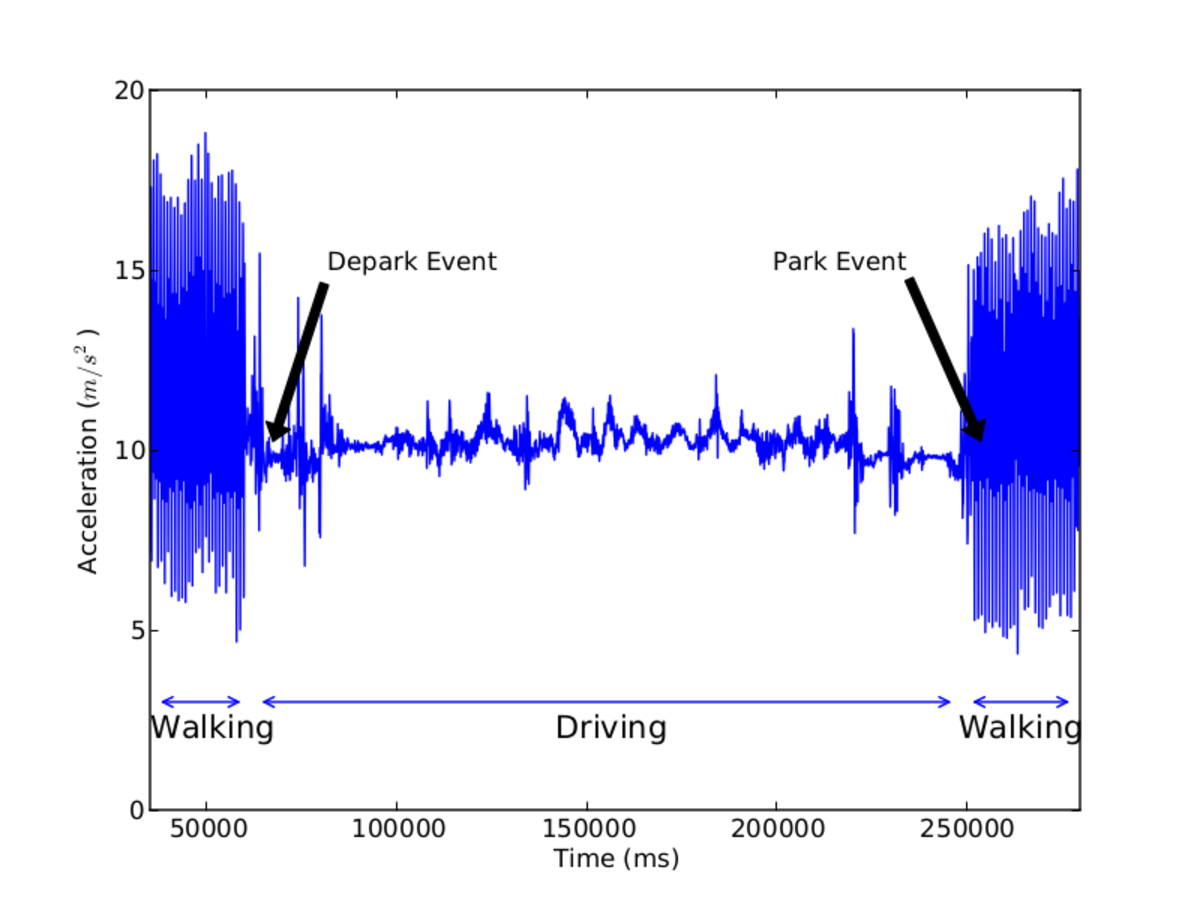
\includegraphics[width=0.8\columnwidth]{./figures/detection-cropped.pdf}

  \caption{\textbf{Detection algorithm.} The graph shows the accelerometer data collected
    during our controlled experiment and shows a period of walking, followed by
    driving, followed by a return to walking. Transitions between these states
  indicate parking lot arrivals and departures.}

  \label{fig-detection}
\end{figure}

\subsection{Parking Events}

PocketParker assumes that transitions between walking and driving that occur
inside known parking lots constitute either arrival (driving to walking) or
departure (walking to driving) events.  We thus must be able to discern
between walking and driving states of the user, and to do so fast enough to
fix the the location of the parking lot in which the event took place.
Detecting these states could be achieved using continuously-sampled GPS data
would consume too much energy for an effective pocketsourcing solution.
Rather, we rely on duty-cycled accelerometer data to classify the user
behavior into one of three states: walking, driving, or idle.

Figure~\ref{fig-detection} depicts two changes in user state, from walking to
driving and back again.  The initial inference of state yielded by the
accelerometer is subsequently refined with GPS and WiFi sense data to yield
the desired goal:  detection of arrival and departure events.  The mobile
device reports these events, along with their locations, to the server.
Before recording the event, the server verifies its location against a list
of known parking lot locations.  This final step eliminates events that are
either obviously incorrect (a user parking in a field) or unwanted (a user
parking but in a loading area rather than in a lot).

After we deployed our PocketParker prototype, Google incorporated activity
recognition algorithms into its Google Play Services library. We have
incorporated their code into PocketParker and, while we have not performed a
detailed evaluation, we have not found the change to affect PocketParker's
event detection accuracy.
